\chapter{Displaying Data from Multiple Tables}

\section{\textbf{Practice 6}}

%--------------------------------------
\subsubsection*{Problem 01}
\addcontentsline{toc}{subsection}{Problem 01}
Write a query for the HR department to produce the addresses of all the departments. Use the LOCATIONS and COUNTRIES tables. Show the location ID, street address, city, state or province, and country in the output. Use a NATURAL JOIN to produce the results.

\begin{frame}

\AddToShipoutPictureFG*{ % Add figure to foreground of current page
  \put(\LenToUnit{5.5cm},\LenToUnit{5cm}){% Adjust the coordinates as needed
    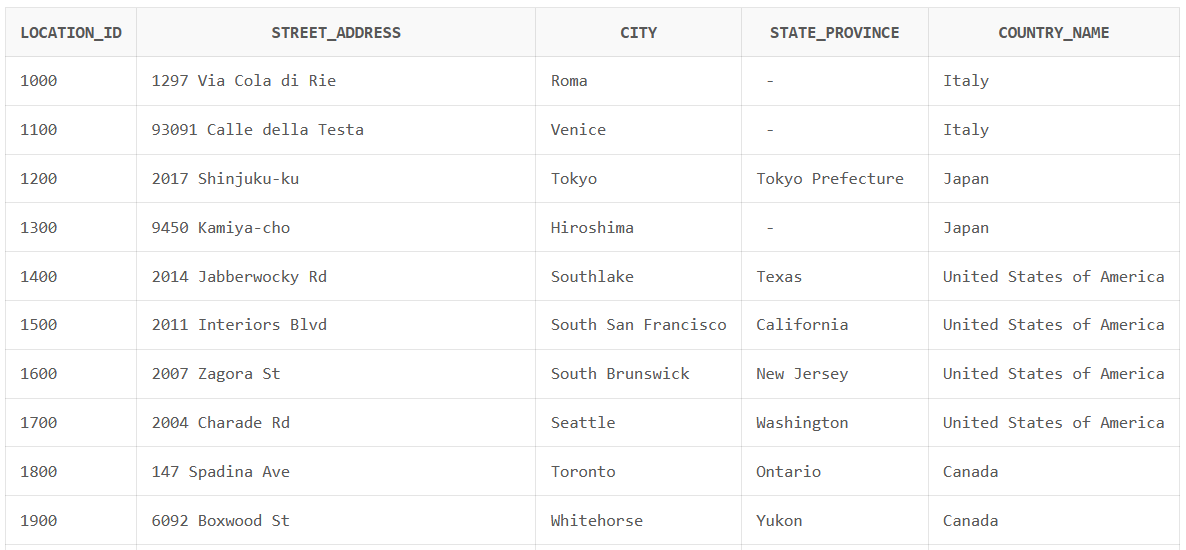
\includegraphics[width=13cm]{Figs/fig_601.png}
  }
}

\lstset{
  basicstyle=\fontsize{10}{12}\selectfont\ttfamily
}

\begin{lstlisting}[language=SQL]
SELECT 	location_id, street_address, city, 
    	state_province, country_name
FROM	hr.locations
NATURAL JOIN hr.countries;
\end{lstlisting}
\textbf{Output: }
\end{frame}


%--------------------------------------
\newpage
\subsubsection*{Problem 02}
\addcontentsline{toc}{subsection}{Problem 02}
The HR department needs a report of all employees. Write a query to display the last name, department number, and department name for all the employees.

\begin{frame}

\AddToShipoutPictureFG*{ % Add figure to foreground of current page
  \put(\LenToUnit{5.5cm},\LenToUnit{14.5cm}){% Adjust the coordinates as needed
    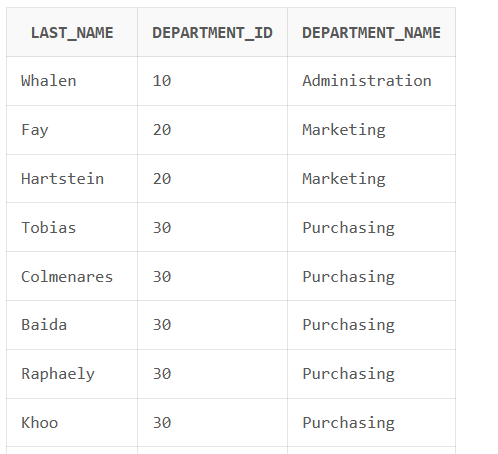
\includegraphics[width=7cm]{Figs/fig_602.png}
  }
}

\lstset{
  basicstyle=\fontsize{10}{12}\selectfont\ttfamily
}

\begin{lstlisting}[language=SQL]
SELECT 	last_name, department_id, department_name
FROM	hr.employees
JOIN	hr.departments USING (department_id);
\end{lstlisting}
\textbf{Output: }
\end{frame}


%--------------------------------------
\vspace{6.5cm}
\subsubsection*{Problem 03}
\addcontentsline{toc}{subsection}{Problem 03}
The HR department needs a report of all employees. Write a query to display the last name, department number, and department name for all the employees.

\begin{frame}

\AddToShipoutPictureFG*{ % Add figure to foreground of current page
  \put(\LenToUnit{5.5cm},\LenToUnit{3cm}){% Adjust the coordinates as needed
    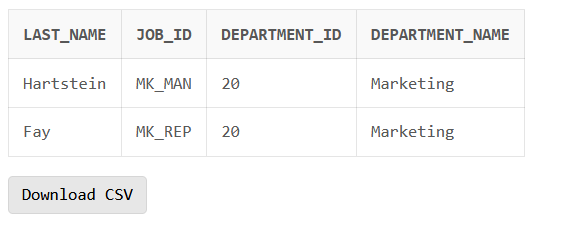
\includegraphics[width=10cm]{Figs/fig_603.png}
  }
}

\lstset{
  basicstyle=\fontsize{10}{12}\selectfont\ttfamily
}

\begin{lstlisting}[language=SQL]
SELECT 	last_name, job_id, department_id, department_name
FROM 	hr.employees
JOIN	hr.departments USING (department_id)
JOIN	hr.locations USING (location_id)
WHERE	city = 'Toronto';
\end{lstlisting}
\textbf{Output: }
\end{frame}

%-----------------------------
\newpage
\subsubsection*{Problem 04}
\addcontentsline{toc}{subsection}{Problem 04}
Create a report to display employees last name and employee number along with their managers last name and manager number. Label the columns Employee, Emp\#, Manager, and Mgr\#, respectively. Run the query.

\begin{frame}

\AddToShipoutPictureFG*{ % Add figure to foreground of current page
  \put(\LenToUnit{13cm},\LenToUnit{15.3cm}){% Adjust the coordinates as needed
    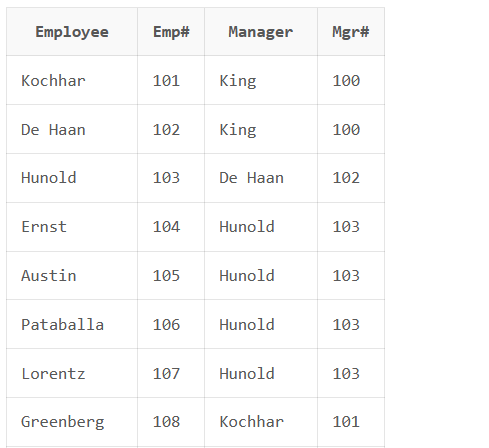
\includegraphics[width=7cm]{Figs/fig_604.png}
  }
}

\lstset{
  basicstyle=\fontsize{10}{12}\selectfont\ttfamily
}

\begin{lstlisting}[language=SQL]
SELECT 	e.last_name AS "Employee",
		e.employee_id AS "Emp#",
		m.last_name AS "Manager",
		m.employee_id AS "Mgr#"
    
FROM	hr.employees e
JOIN	hr.employees m 
		ON (e.manager_id = m.employee_id)
ORDER BY	e.employee_id;
\end{lstlisting}
\textbf{Output: }
\end{frame}

%----------------------------
\vspace{0.5cm}
\subsubsection*{Problem 05}
\addcontentsline{toc}{subsection}{Problem 05}
Modify lab\_06\_04.sql to display all employees including King, who has no manager. Order the results by the employee number. Save your SQL statement as lab\_06\_05.sql. Run the query in lab\_06\_05.sql.

\begin{frame}

\AddToShipoutPictureFG*{ % Add figure to foreground of current page
  \put(\LenToUnit{5.5cm},\LenToUnit{2.3cm}){% Adjust the coordinates as needed
    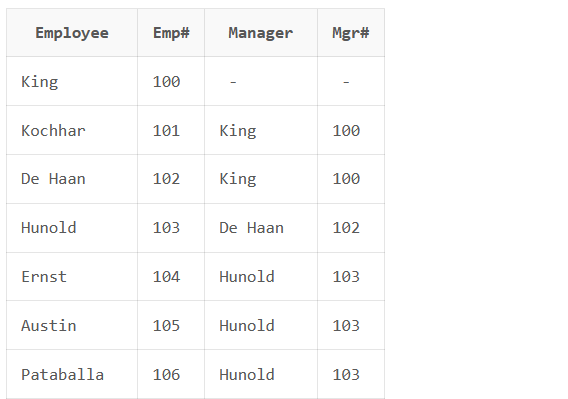
\includegraphics[width=9cm]{Figs/fig_605.png}
  }
}

\lstset{
  basicstyle=\fontsize{10}{12}\selectfont\ttfamily
}

\begin{lstlisting}[language=SQL]
SELECT e.last_name AS "Employee",
       e.employee_id AS "Emp#",
       m.last_name AS "Manager",
       m.employee_id AS "Mgr#"
FROM   hr.employees e
LEFT JOIN hr.employees m ON (e.manager_id = m.employee_id)
ORDER BY e.employee_id;
\end{lstlisting}
\textbf{Output: }
\end{frame}


%-----------------------------
\newpage
\subsubsection*{Problem 06}
\addcontentsline{toc}{subsection}{Problem 06}
Create a report for the HR department that displays employee last names, department numbers, and all the employees who work in the same department as a given employee. Give each column an appropriate label. Save the script to a file named lab\_06\_06.sql.

\begin{frame}

\AddToShipoutPictureFG*{ % Add figure to foreground of current page
  \put(\LenToUnit{13cm},\LenToUnit{12.5cm}){% Adjust the coordinates as needed
    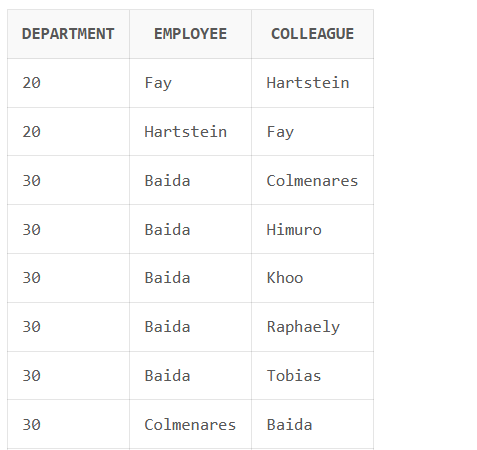
\includegraphics[width=7cm]{Figs/fig_606.png}
  }
}

\lstset{
  basicstyle=\fontsize{10}{12}\selectfont\ttfamily
}

\begin{lstlisting}[language=SQL]
SELECT 	e.department_id AS department,
       	e.last_name AS employee,
       	c.last_name AS colleague
FROM 	hr.employees e
JOIN 	hr.employees c ON (e.department_id = c.department_id)
WHERE 	e.employee_id <> c.employee_id
ORDER BY department, employee, colleague;
\end{lstlisting}
\textbf{Output: }
\end{frame}

%---------------------------
\vspace{4cm}
\subsubsection*{Problem 08}
\addcontentsline{toc}{subsection}{Problem 08}
The HR department wants to determine the names of all the employees who were hired after Davies. Create a query to display the name and hire date of any employee hired after employee Davies.
\begin{frame}

\AddToShipoutPictureFG*{ % Add figure to foreground of current page
  \put(\LenToUnit{5.5cm},\LenToUnit{2.3cm}){% Adjust the coordinates as needed
    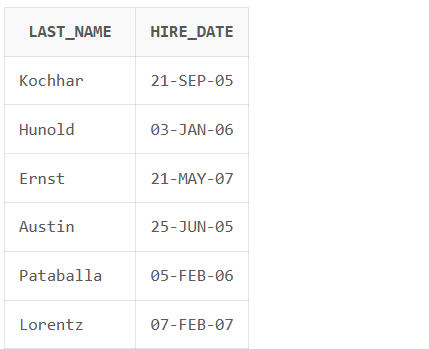
\includegraphics[width=7cm]{Figs/fig_608.png}
  }
}

\lstset{
  basicstyle=\fontsize{10}{12}\selectfont\ttfamily
}

\begin{lstlisting}[language=SQL]
SELECT 	e.last_name,
       	TO_CHAR (e.hire_date, 'DD-MON-YY') hire_date
FROM 	hr.employees e
JOIN 	hr.employees davies ON (davies.last_name = 'Davies')
WHERE 	davies.hire_date < e.hire_date;
\end{lstlisting}
\textbf{Output: }
\end{frame}


%-----------------------------
\newpage
\subsubsection*{Problem 09}
\addcontentsline{toc}{subsection}{Problem 09}
The HR department needs to find the names and hire dates of all the employees who were hired before their managers, along with their managers names and hire dates. Save the script to a file named lab\_06\_09.sql.

\begin{frame}

\AddToShipoutPictureFG*{ % Add figure to foreground of current page
  \put(\LenToUnit{5.5cm},\LenToUnit{10.2cm}){% Adjust the coordinates as needed
    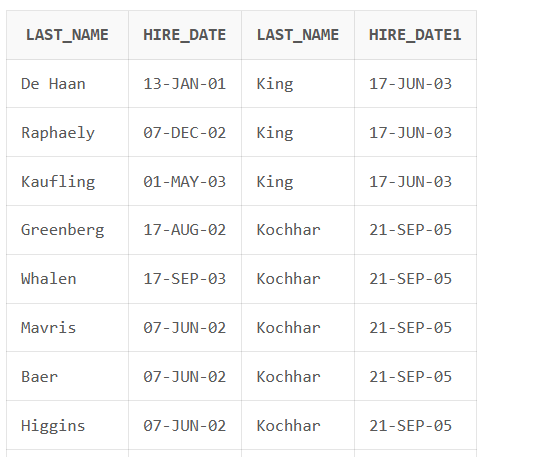
\includegraphics[width=9cm]{Figs/fig_609.png}
  }
}

\lstset{
  basicstyle=\fontsize{10}{12}\selectfont\ttfamily
}

\begin{lstlisting}[language=SQL]
SELECT 	e.last_name,
       	TO_CHAR (e.hire_date, 'DD-MON-YY') hire_date,
       	m.last_name,
       	TO_CHAR (m.hire_date, 'DD-MON-YY') hire_date1
FROM 	hr.employees e
JOIN 	hr.employees m ON (e.manager_id = m.employee_id)
WHERE 	e.hire_date < m.hire_date;
\end{lstlisting}
\textbf{Output: }
\end{frame}


